\documentclass[a4paper,10pt]{beamer}
\usepackage[utf8x]{inputenc}
\usepackage[T1]{fontenc}
\usepackage[english]{babel}
\usepackage{hyperref,graphicx}
\usetheme{Berkeley}

\setbeamertemplate{navigation symbols}{\insertframenumber /\inserttotalframenumber}

\title{3D object from a 2D drawing}
\author[Groupe 3INFO]{Aurélien Fontaine, Manutea Huang, Etienne Geantet,\\ Arnaud Martin}
\institute[INSA de Rennes]{Institut National des Sciences Appliquées de Rennes}
\date{\today}

\begin{document}
	\begin{frame}
		\begin{titlepage}
			\centerline{
\includegraphics[scale=0.1]{images/logos/logoINSA.jpg}}
			Supervisors : François Lehericey and Bertrand Coüasnon	
		\end{titlepage}
	\end{frame}
	
	\begin{frame}
		\tableofcontents
	\end{frame}
	
	\section{Introduction}
	
		\subsection{Our subject}
	
			\begin{frame}{The subject}
				\begin{itemize}
					\item Create an object from a drawing on a tablet
					\item Easy to use: <1min to create a new object
				\end{itemize}
				Final objective : Occupy a room with simple objects made by an user
			\end{frame}
			
		\subsection{Existing technologies}
			
			\begin{frame}{A project made by Sony}
				Project PS4 : The PlayRoom (actually available)
				\href{run:The_PlayRoom.avi}{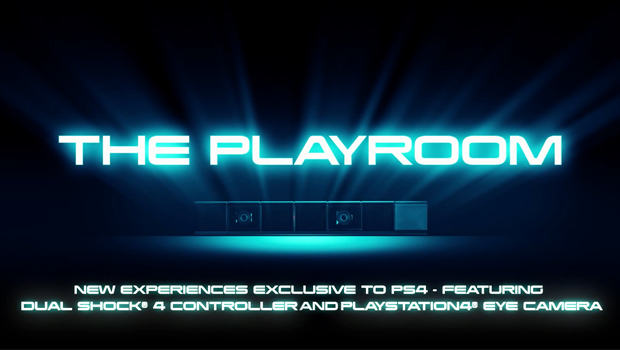
\includegraphics[width=300pt]{images/The-Playroom.jpg}}
			\end{frame}
			
			\begin{frame}{Drawing editors}
				\begin{itemize}
					\item A lot of drawing editors : Markers, LayerPaint, SketchBook, ...
					\item Great drawings
					\item No possibility of making a 3D object
					\item Source code inaccessible
				\end{itemize}
			\end{frame}
	
	\section{Our graphic solution}
		\subsection{Specifications}
		
		\begin{frame}{Specifications}
			\begin{itemize}
				\item A simple and ergonomic application
				\item A tablet application
				\item The exportation have to be compatible with Unity
				\item Create 3D objects more or less complex (simple balloon, or a car with its wheels)
			\end{itemize}
		\end{frame}
		
		\subsection{The interface}
		
			\begin{frame}{The app}
				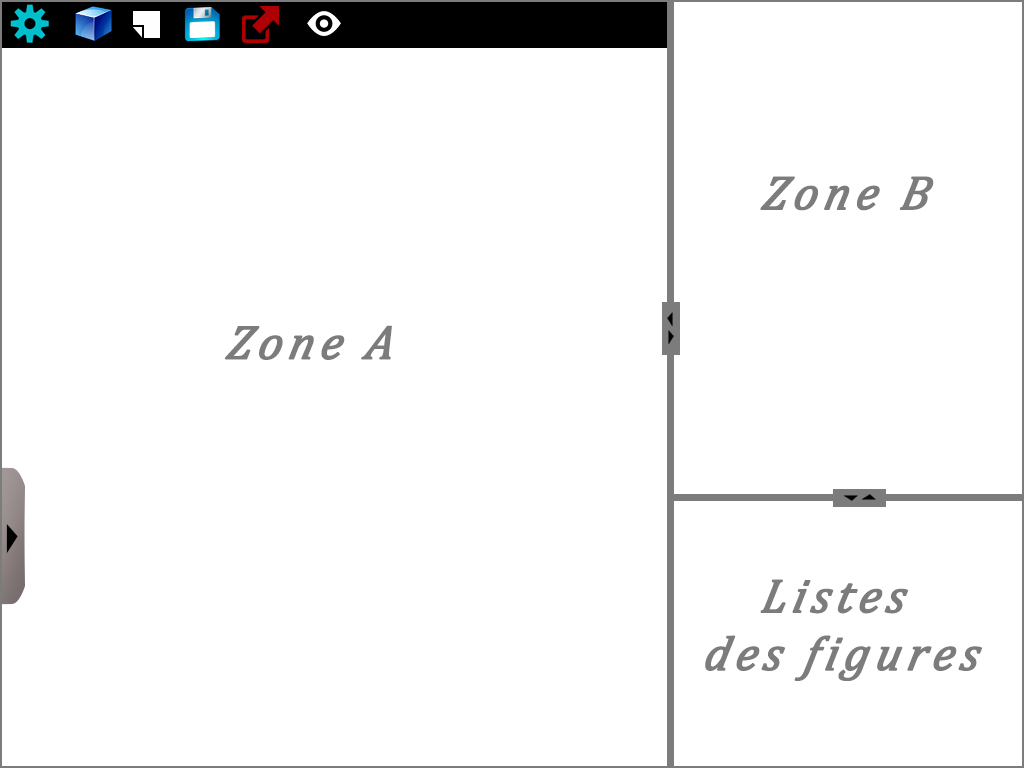
\includegraphics[height=205pt]{maquette/maquette_1.png}
			\end{frame}
			
			\begin{frame}{The app}
				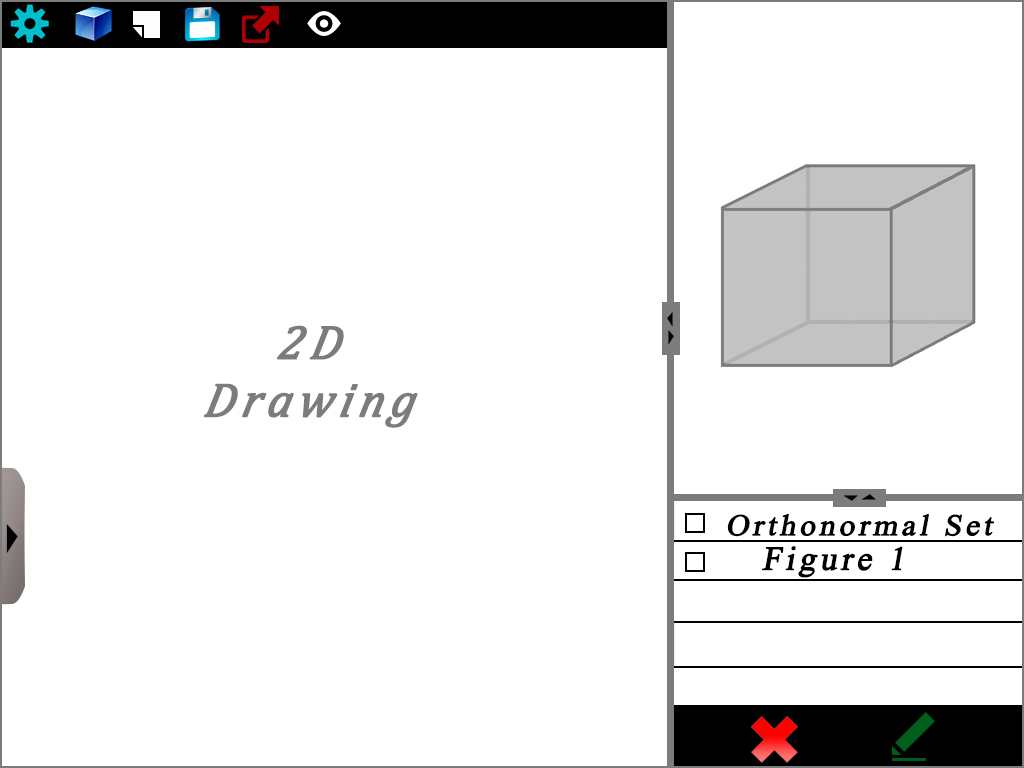
\includegraphics[height=205pt]{maquette/maquette_2.png}
			\end{frame}
			
			\begin{frame}{The app}
				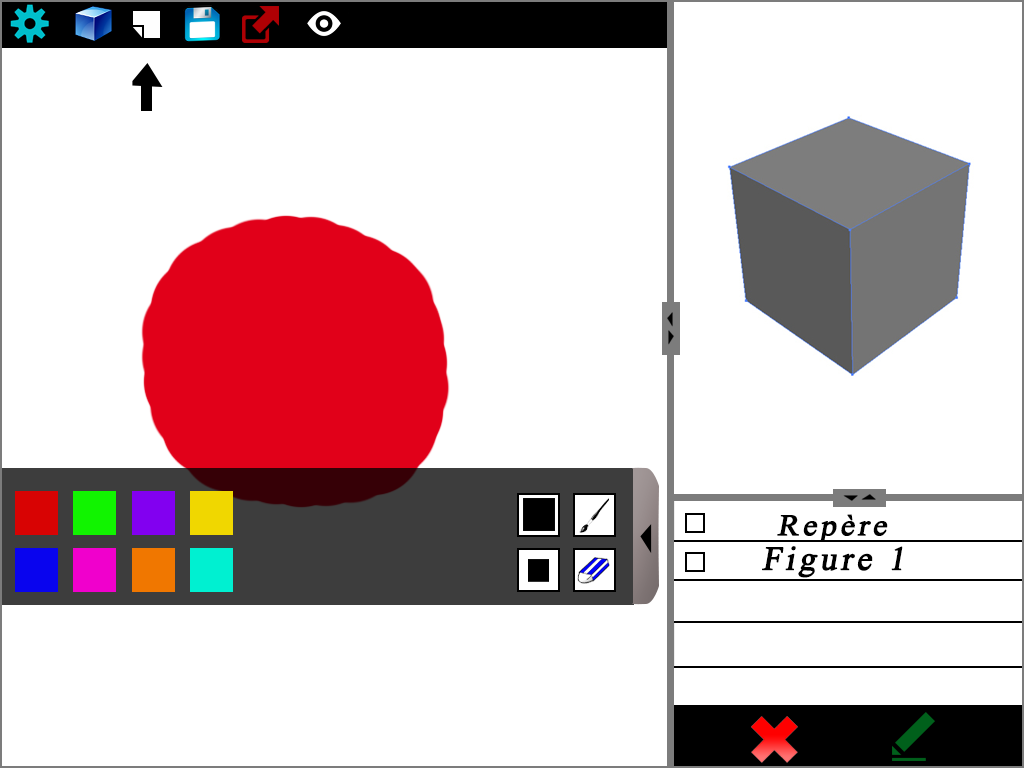
\includegraphics[height=205pt]{maquette/maquette_3.png}
			\end{frame}
			
			\begin{frame}{The app}
				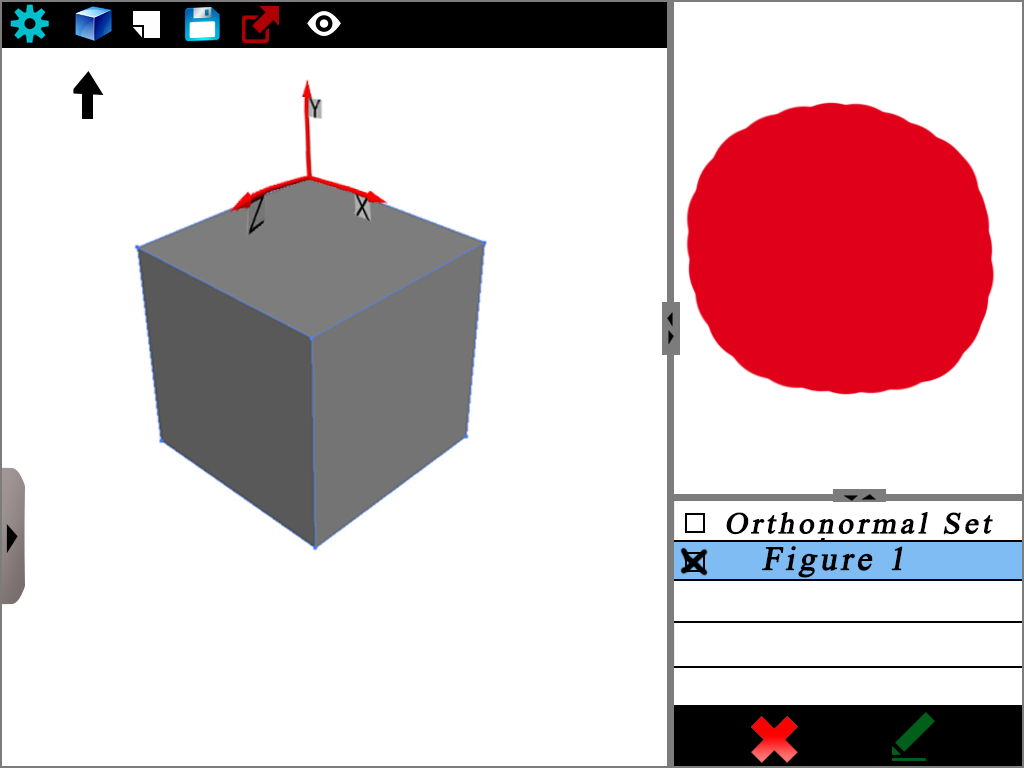
\includegraphics[height=205pt]{maquette/maquette_4.png}
			\end{frame}
			
			\begin{frame}{The app}
				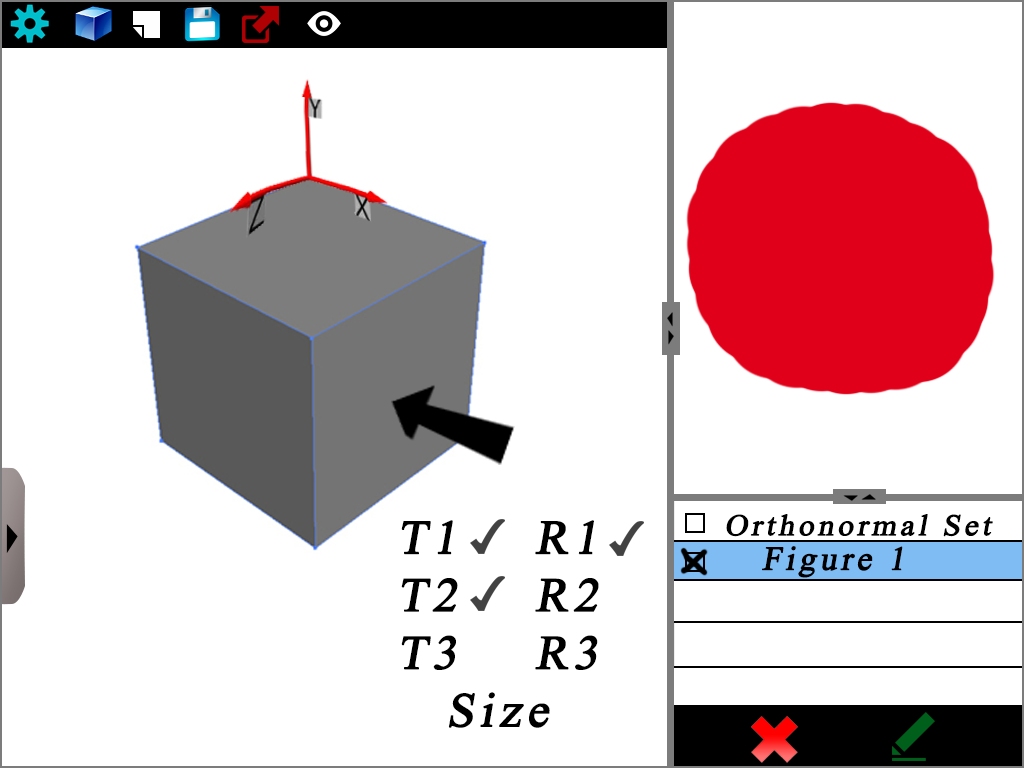
\includegraphics[height=205pt]{maquette/maquette_5.png}
			\end{frame}
			
			\begin{frame}{The app}
				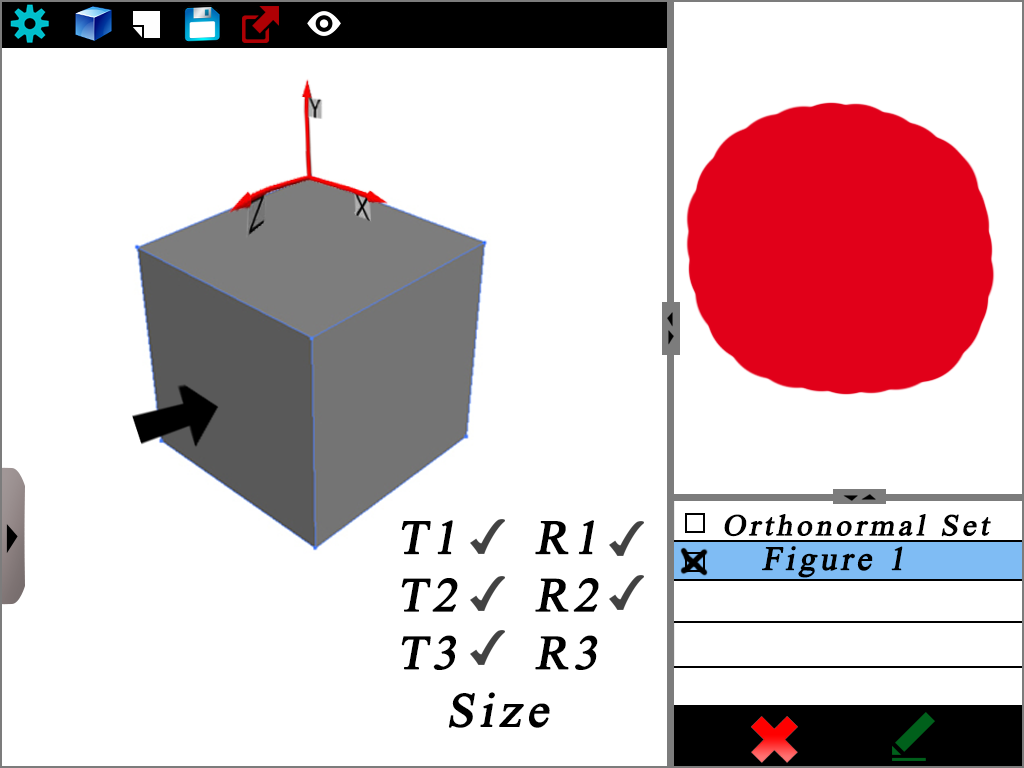
\includegraphics[height=205pt]{maquette/maquette_6.png}
			\end{frame}
			
			\begin{frame}{The app}
				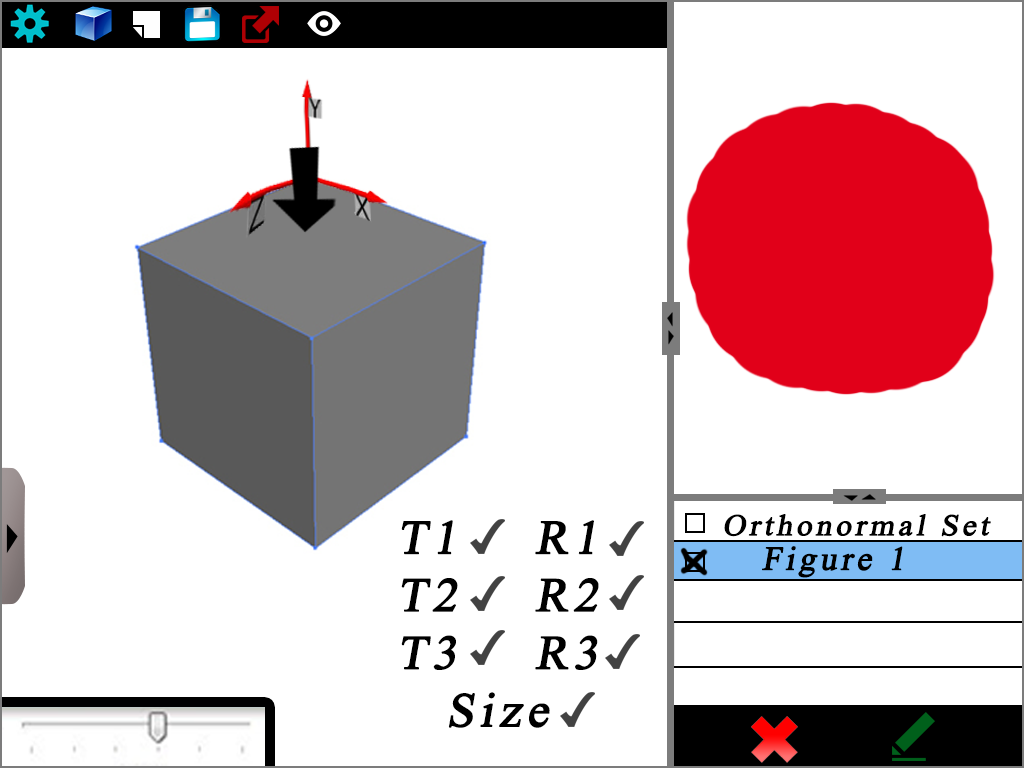
\includegraphics[height=205pt]{maquette/maquette_7.png}
			\end{frame}
			
			\begin{frame}{The app}
				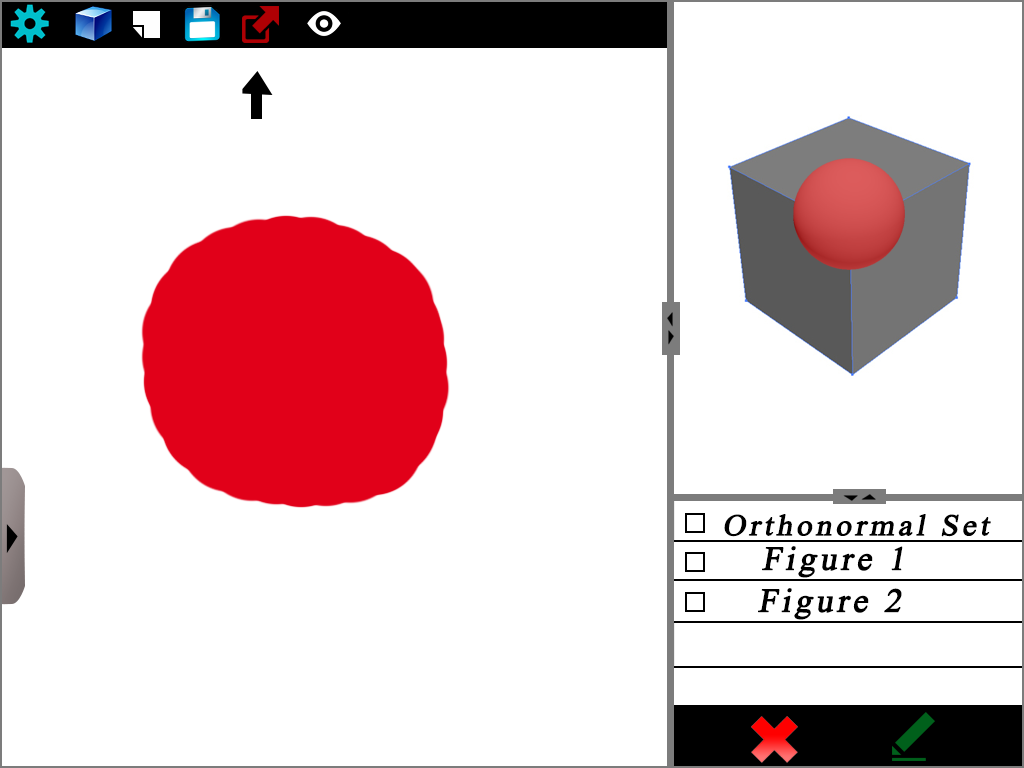
\includegraphics[height=205pt]{maquette/maquette_8.png}
			\end{frame}
	
	\section{The technology : the engine}
	
		
			
		\subsection{Some existing 3D engines}
		
			\begin{frame}{Unreal Engine}
				
\includegraphics[height=120pt]{images/logos/Unreal_Engine.png}\\
				A game engine made for FPS
				\begin{itemize}
					\item Few help to develop on tablets
					\item Have to go around for simple tasks (the interface = a pause menu)
				\end{itemize}
			\end{frame}
			
			\begin{frame}{CryEngine}
				
\includegraphics[height=100pt]{images/logos/Cry_Engine.png}
			\end{frame}
			
			\begin{frame}{OpenGl}
				
\includegraphics[height=75pt]{images/logos/OpenGL_logo.png}
				\begin{itemize}
					\item A language hardware oriented (hard to change of devices)
					\item A long time to learn how to use it
					\item A lot of code lines just for a simple form
				\end{itemize}
			\end{frame}
			
			\begin{frame}{Autodesk Maya}
				
\includegraphics[height=75pt]{images/logos/Autodesk_Maya.png}
			\end{frame}
			
		\subsection{Unity}
		
			\begin{frame}{Unity}
				
\includegraphics[height=75pt]{images/logos/Logo_Unity.jpg}
				\begin{itemize}
					\item now free
					\item entity oriented
					\item easier then others to learn
				\end{itemize}
			\end{frame}
			
			\begin{frame}{Unity : A large compatibility}
				Over 15 different platforms :\\
				\\
				\begin{itemize}
					\item Os :
				\end{itemize}
				
\includegraphics[height=30pt]{images/PlatformesDesktop.png}
				
				\begin{itemize}
					\item Tablets :
				\end{itemize}
				
\includegraphics[height=30pt]{images/PlatformesTabPhones.png}
			\end{frame}	
			
			\begin{frame}{Our Choice}
				We have chosen Unity for multiple reasons :
				\begin{itemize}
					\item Easy to use on different OS
					\item An engine very powerful with a few lines
					\item The exportation between two devices under Unity is simple
				\end{itemize}			
			\end{frame}
		
	\section{Network}
		
		\begin{frame}{Network}
			\centerline{
\includegraphics[height=205pt]{images/network/network.png}}
		\end{frame}
		
		\subsection{How does it work?}
		
			\begin{frame}{How does it work?}
				\centerline{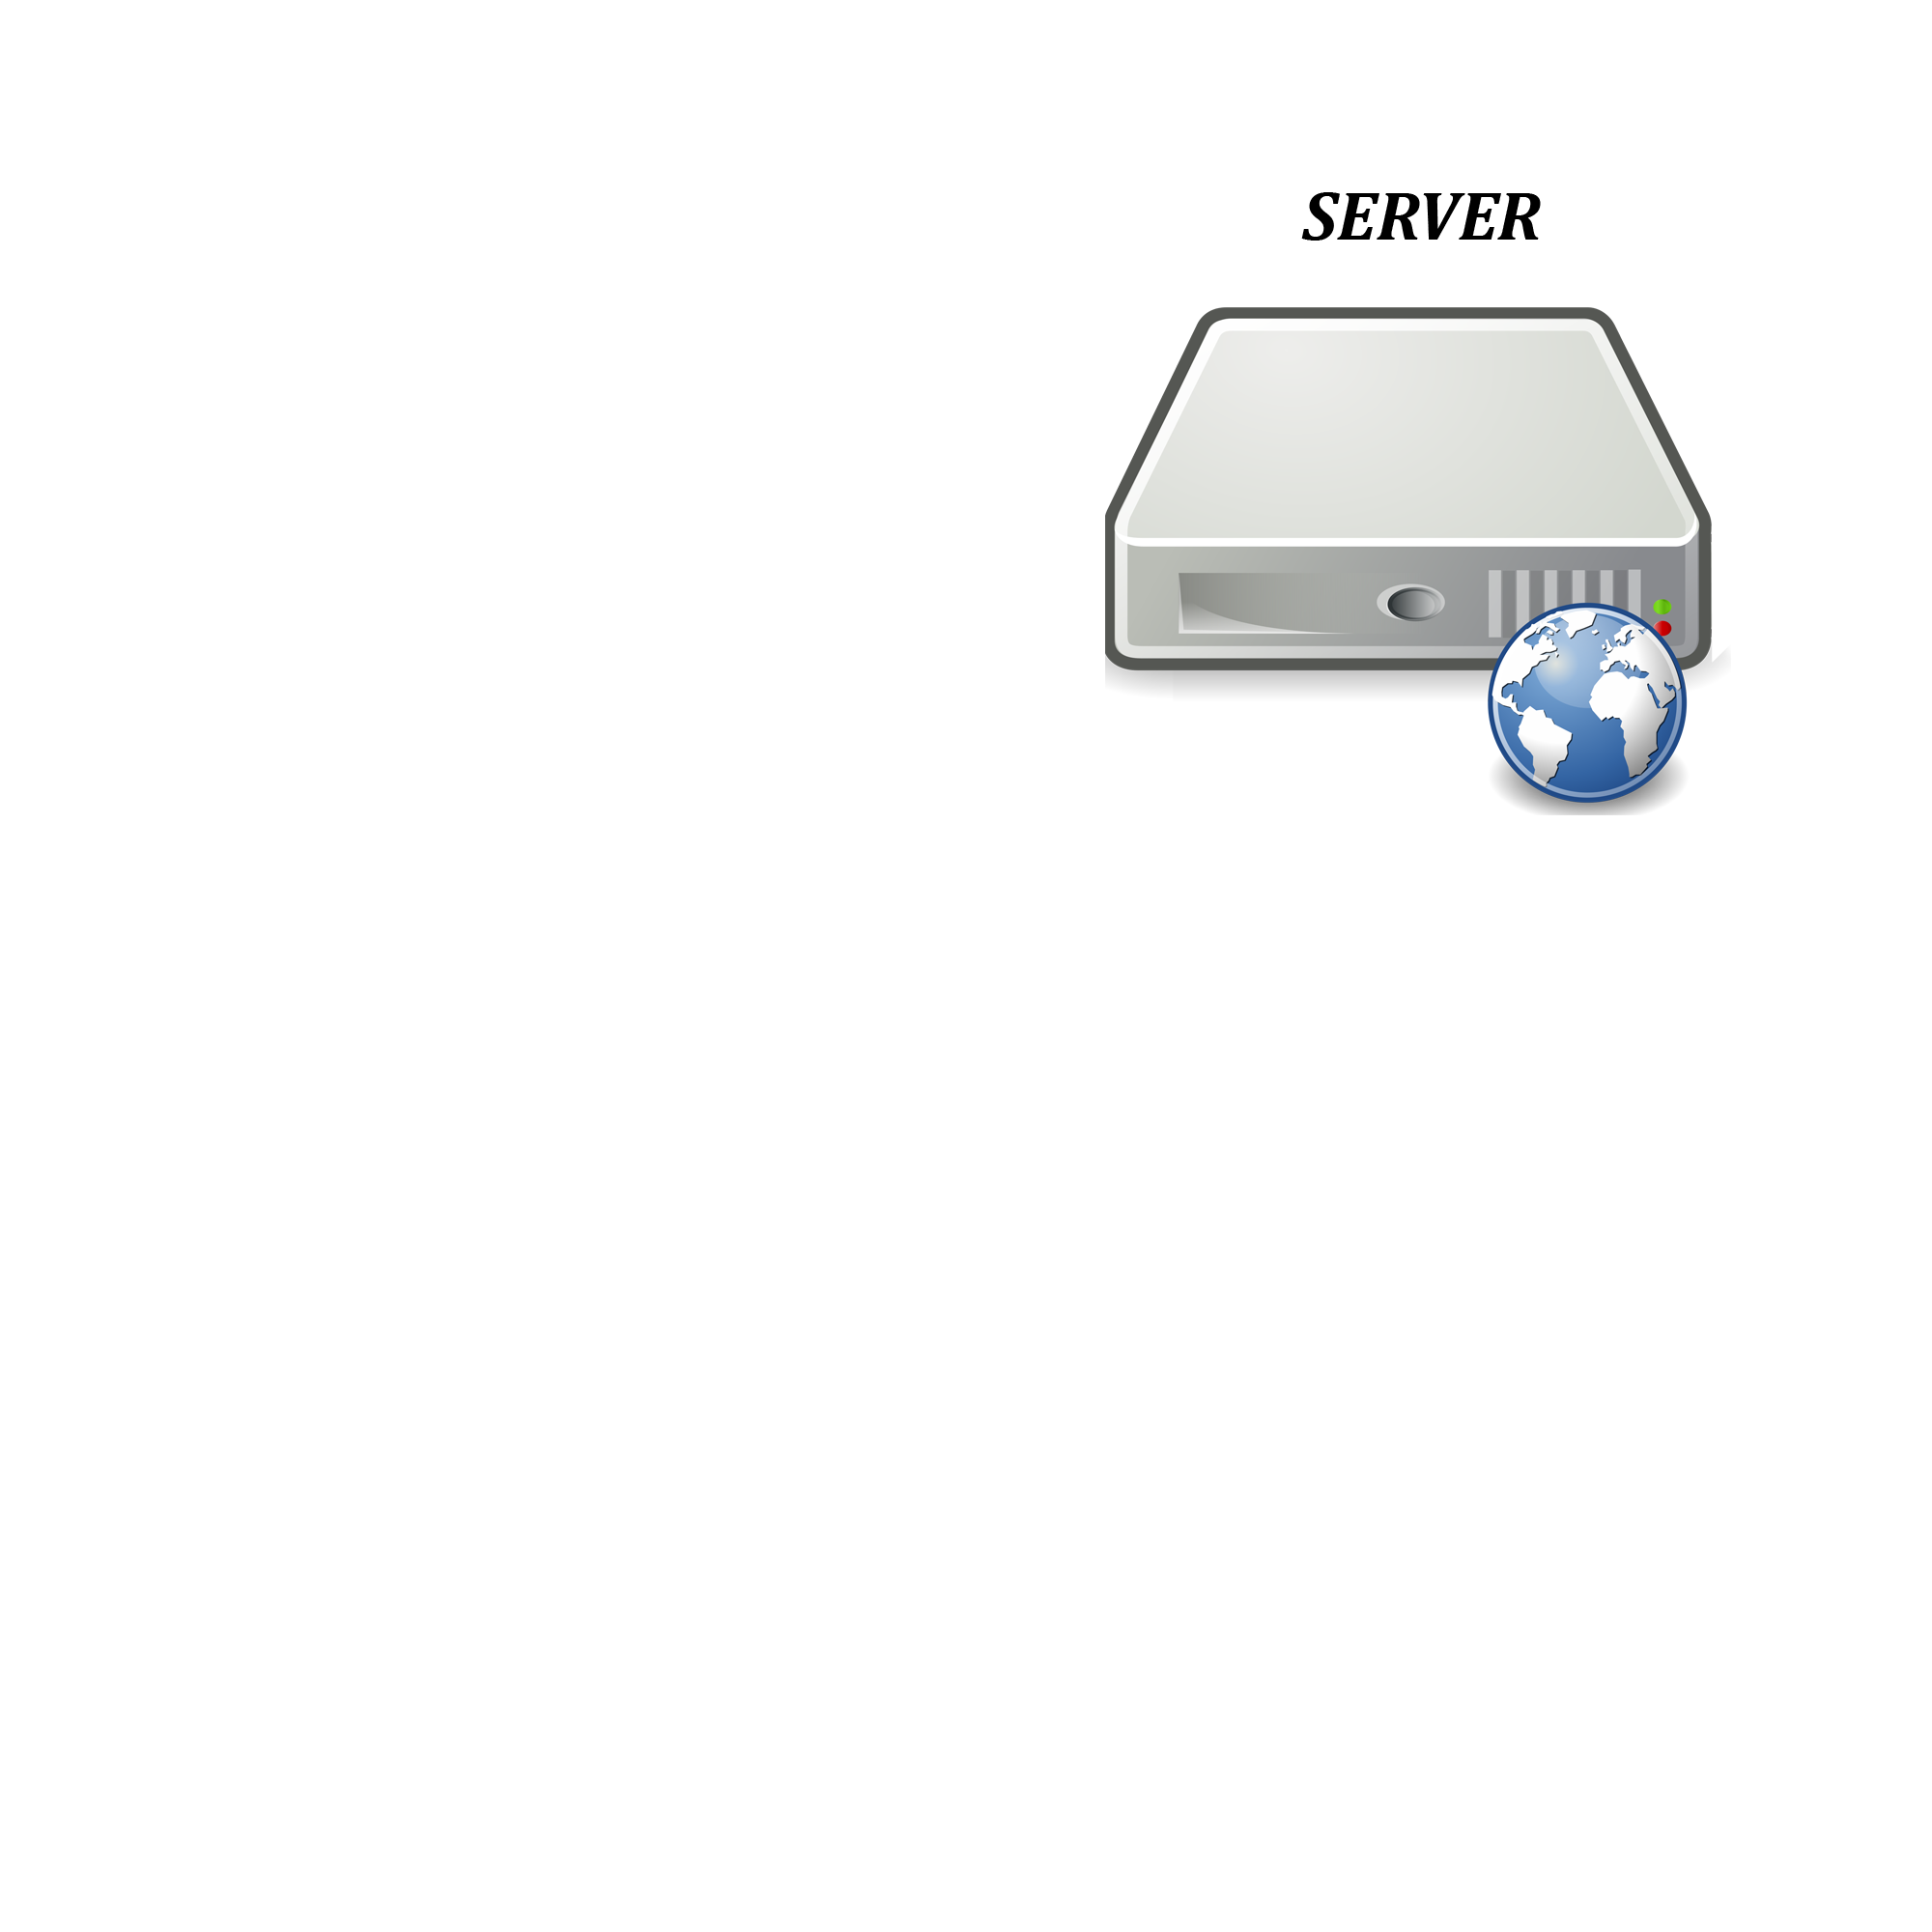
\includegraphics[height=205pt]{images/network/server.png}}
			\end{frame}
		
			\begin{frame}{How does it work?}
				\centerline{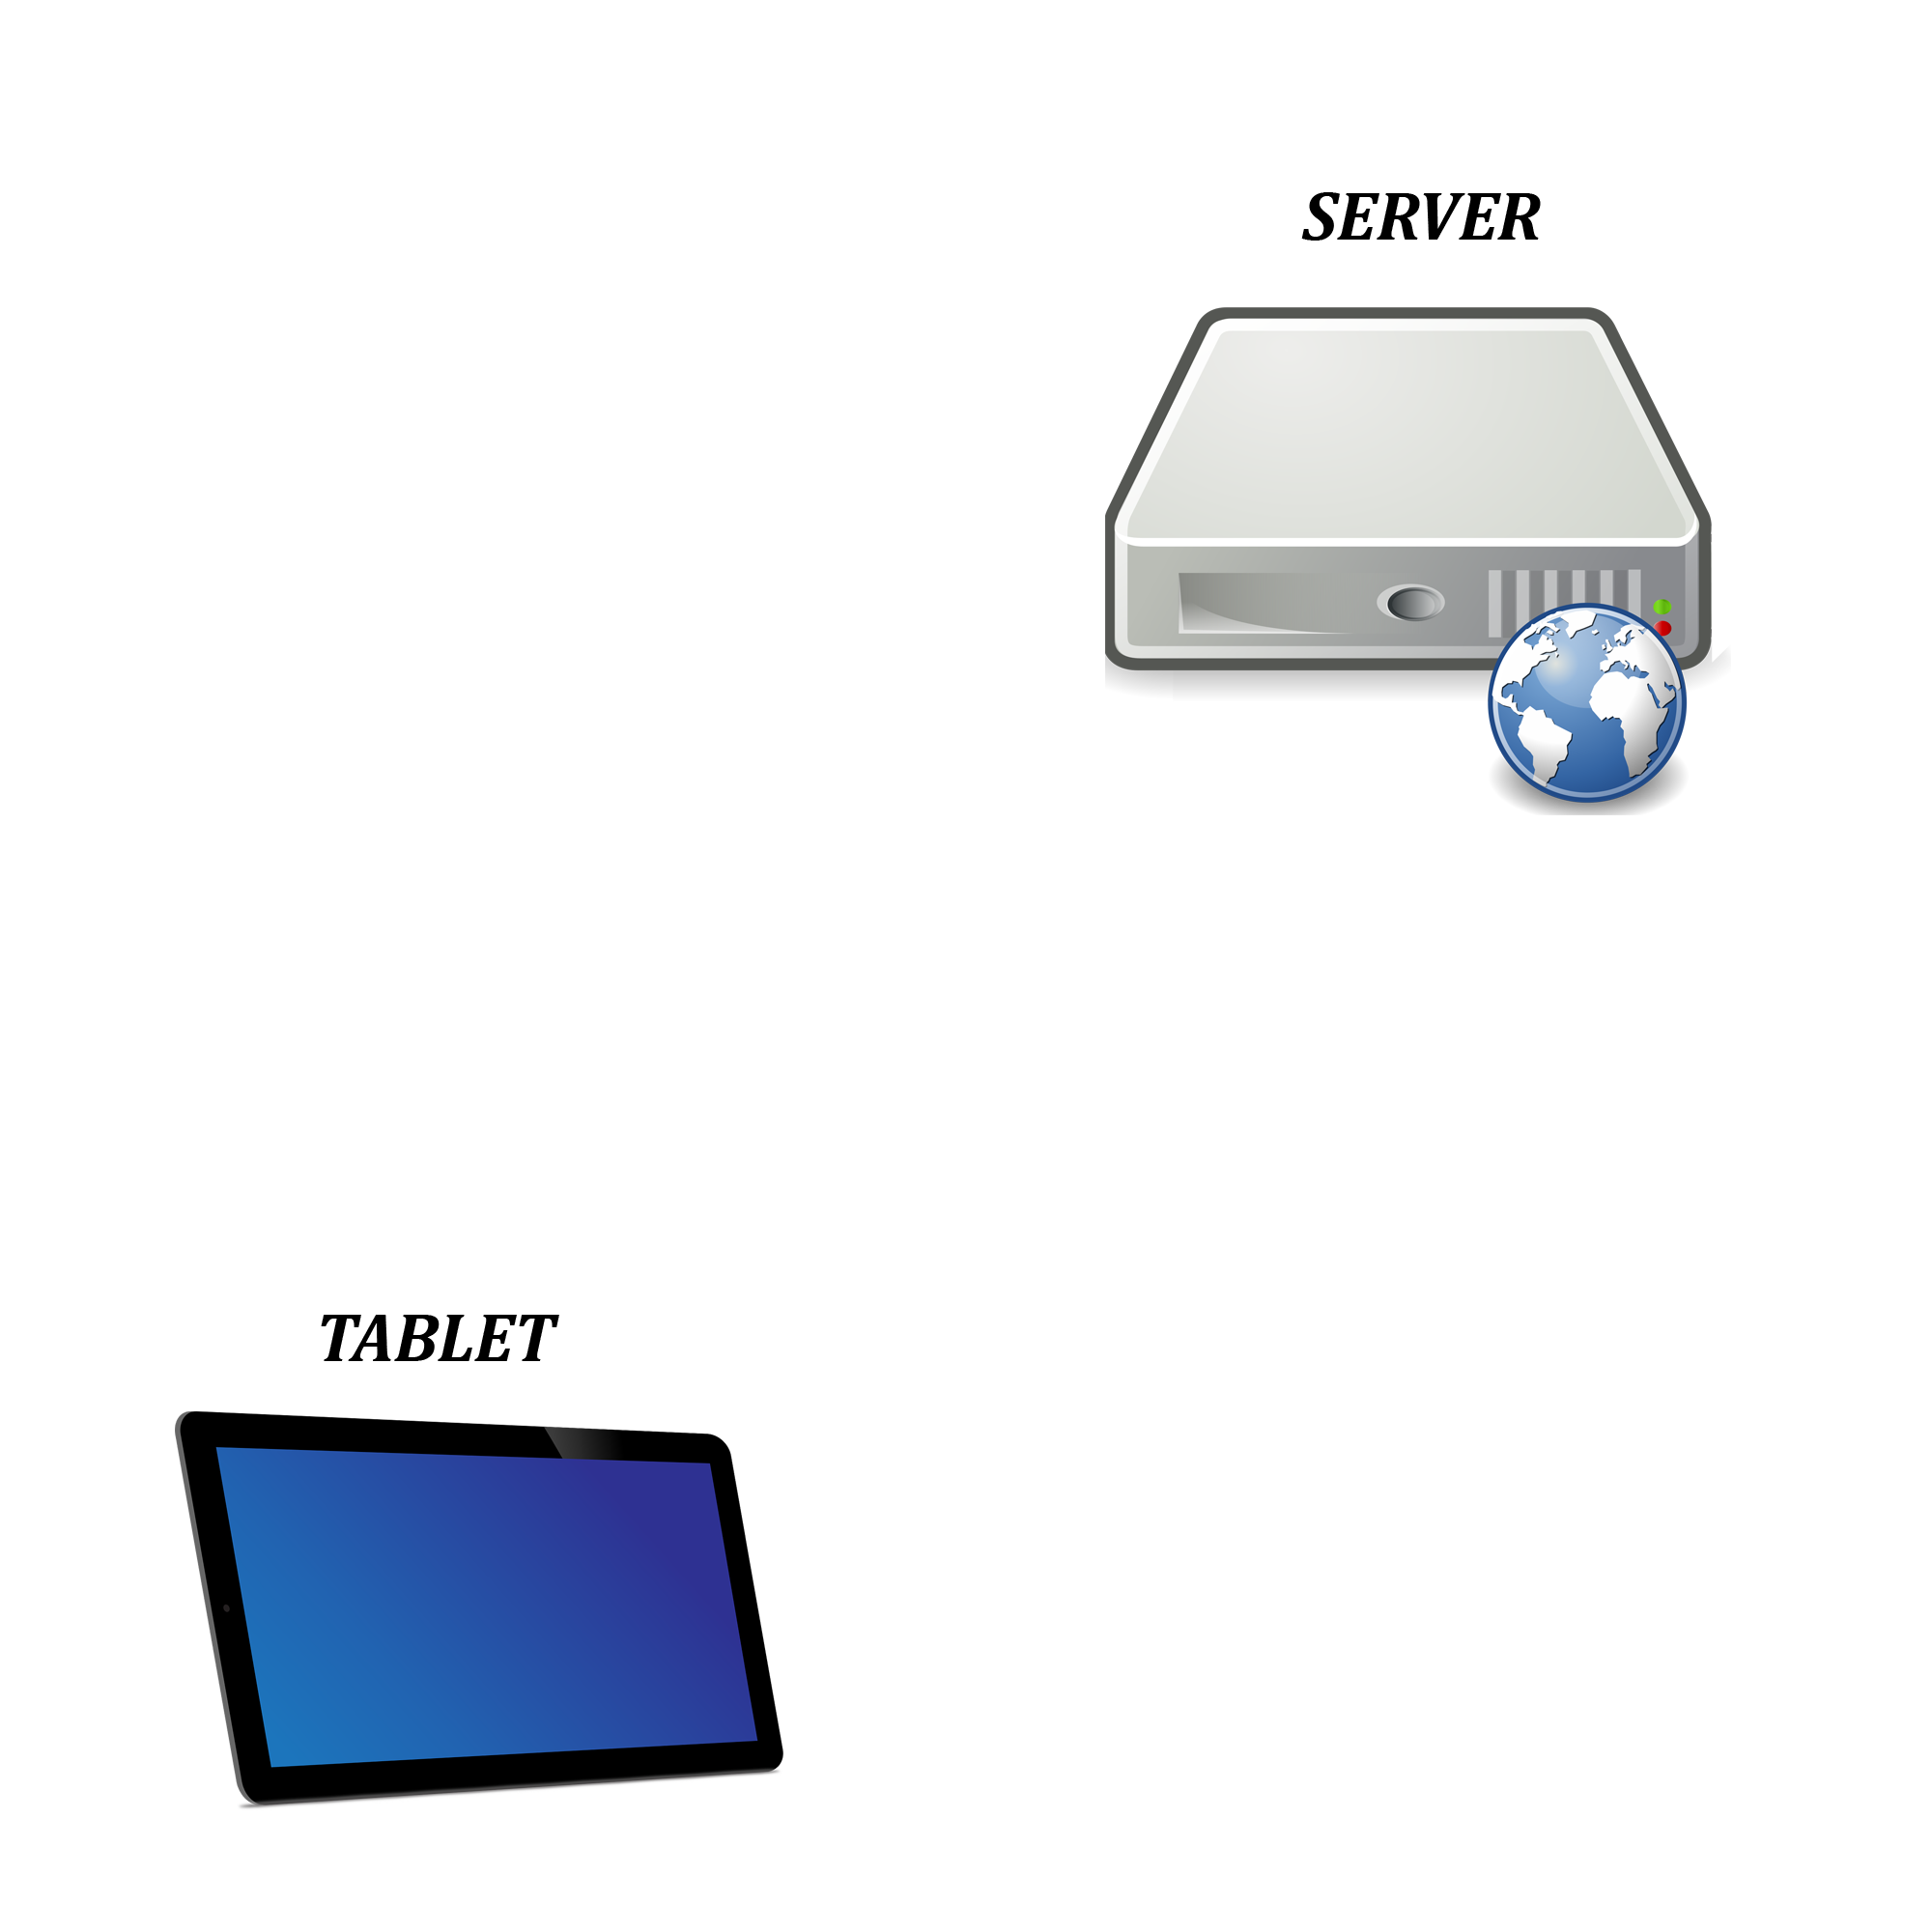
\includegraphics[height=205pt]{images/network/tabletandserver.png}}
			\end{frame}
		
			\begin{frame}{How does it work?}
				\centerline{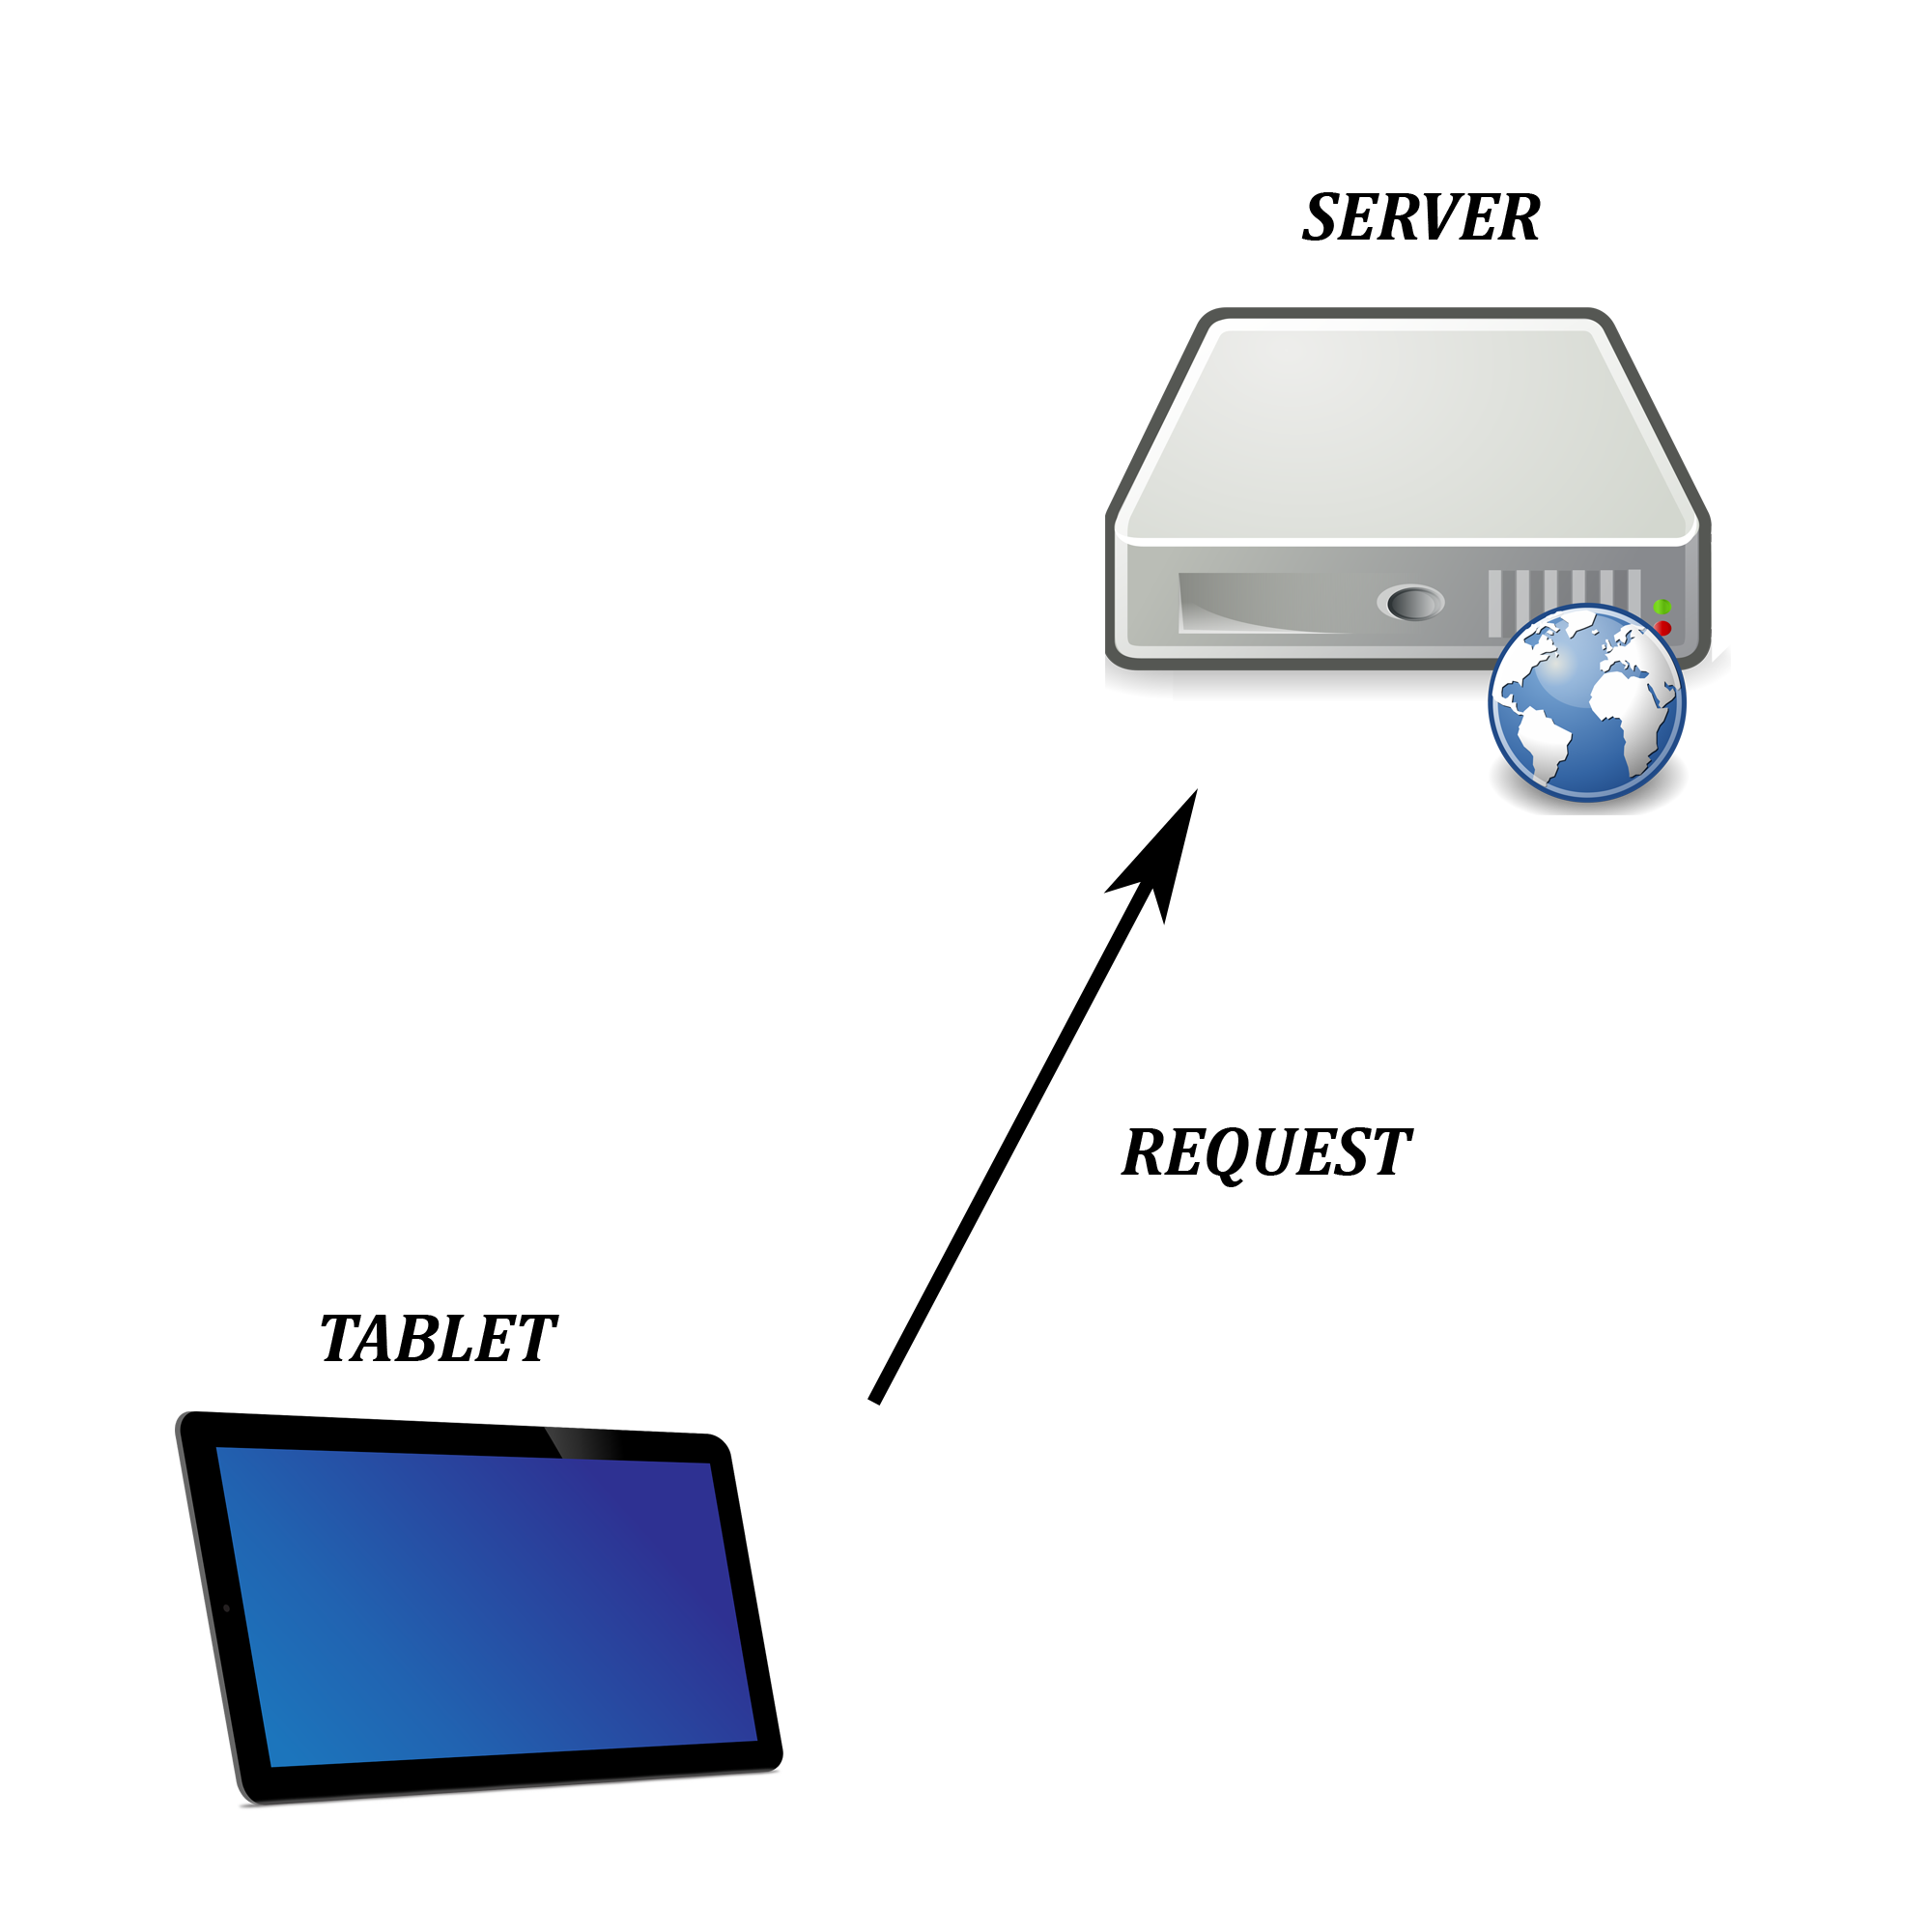
\includegraphics[height=205pt]{images/network/request.png}}
			\end{frame}
			
			\begin{frame}{How does it work?}
				\centerline{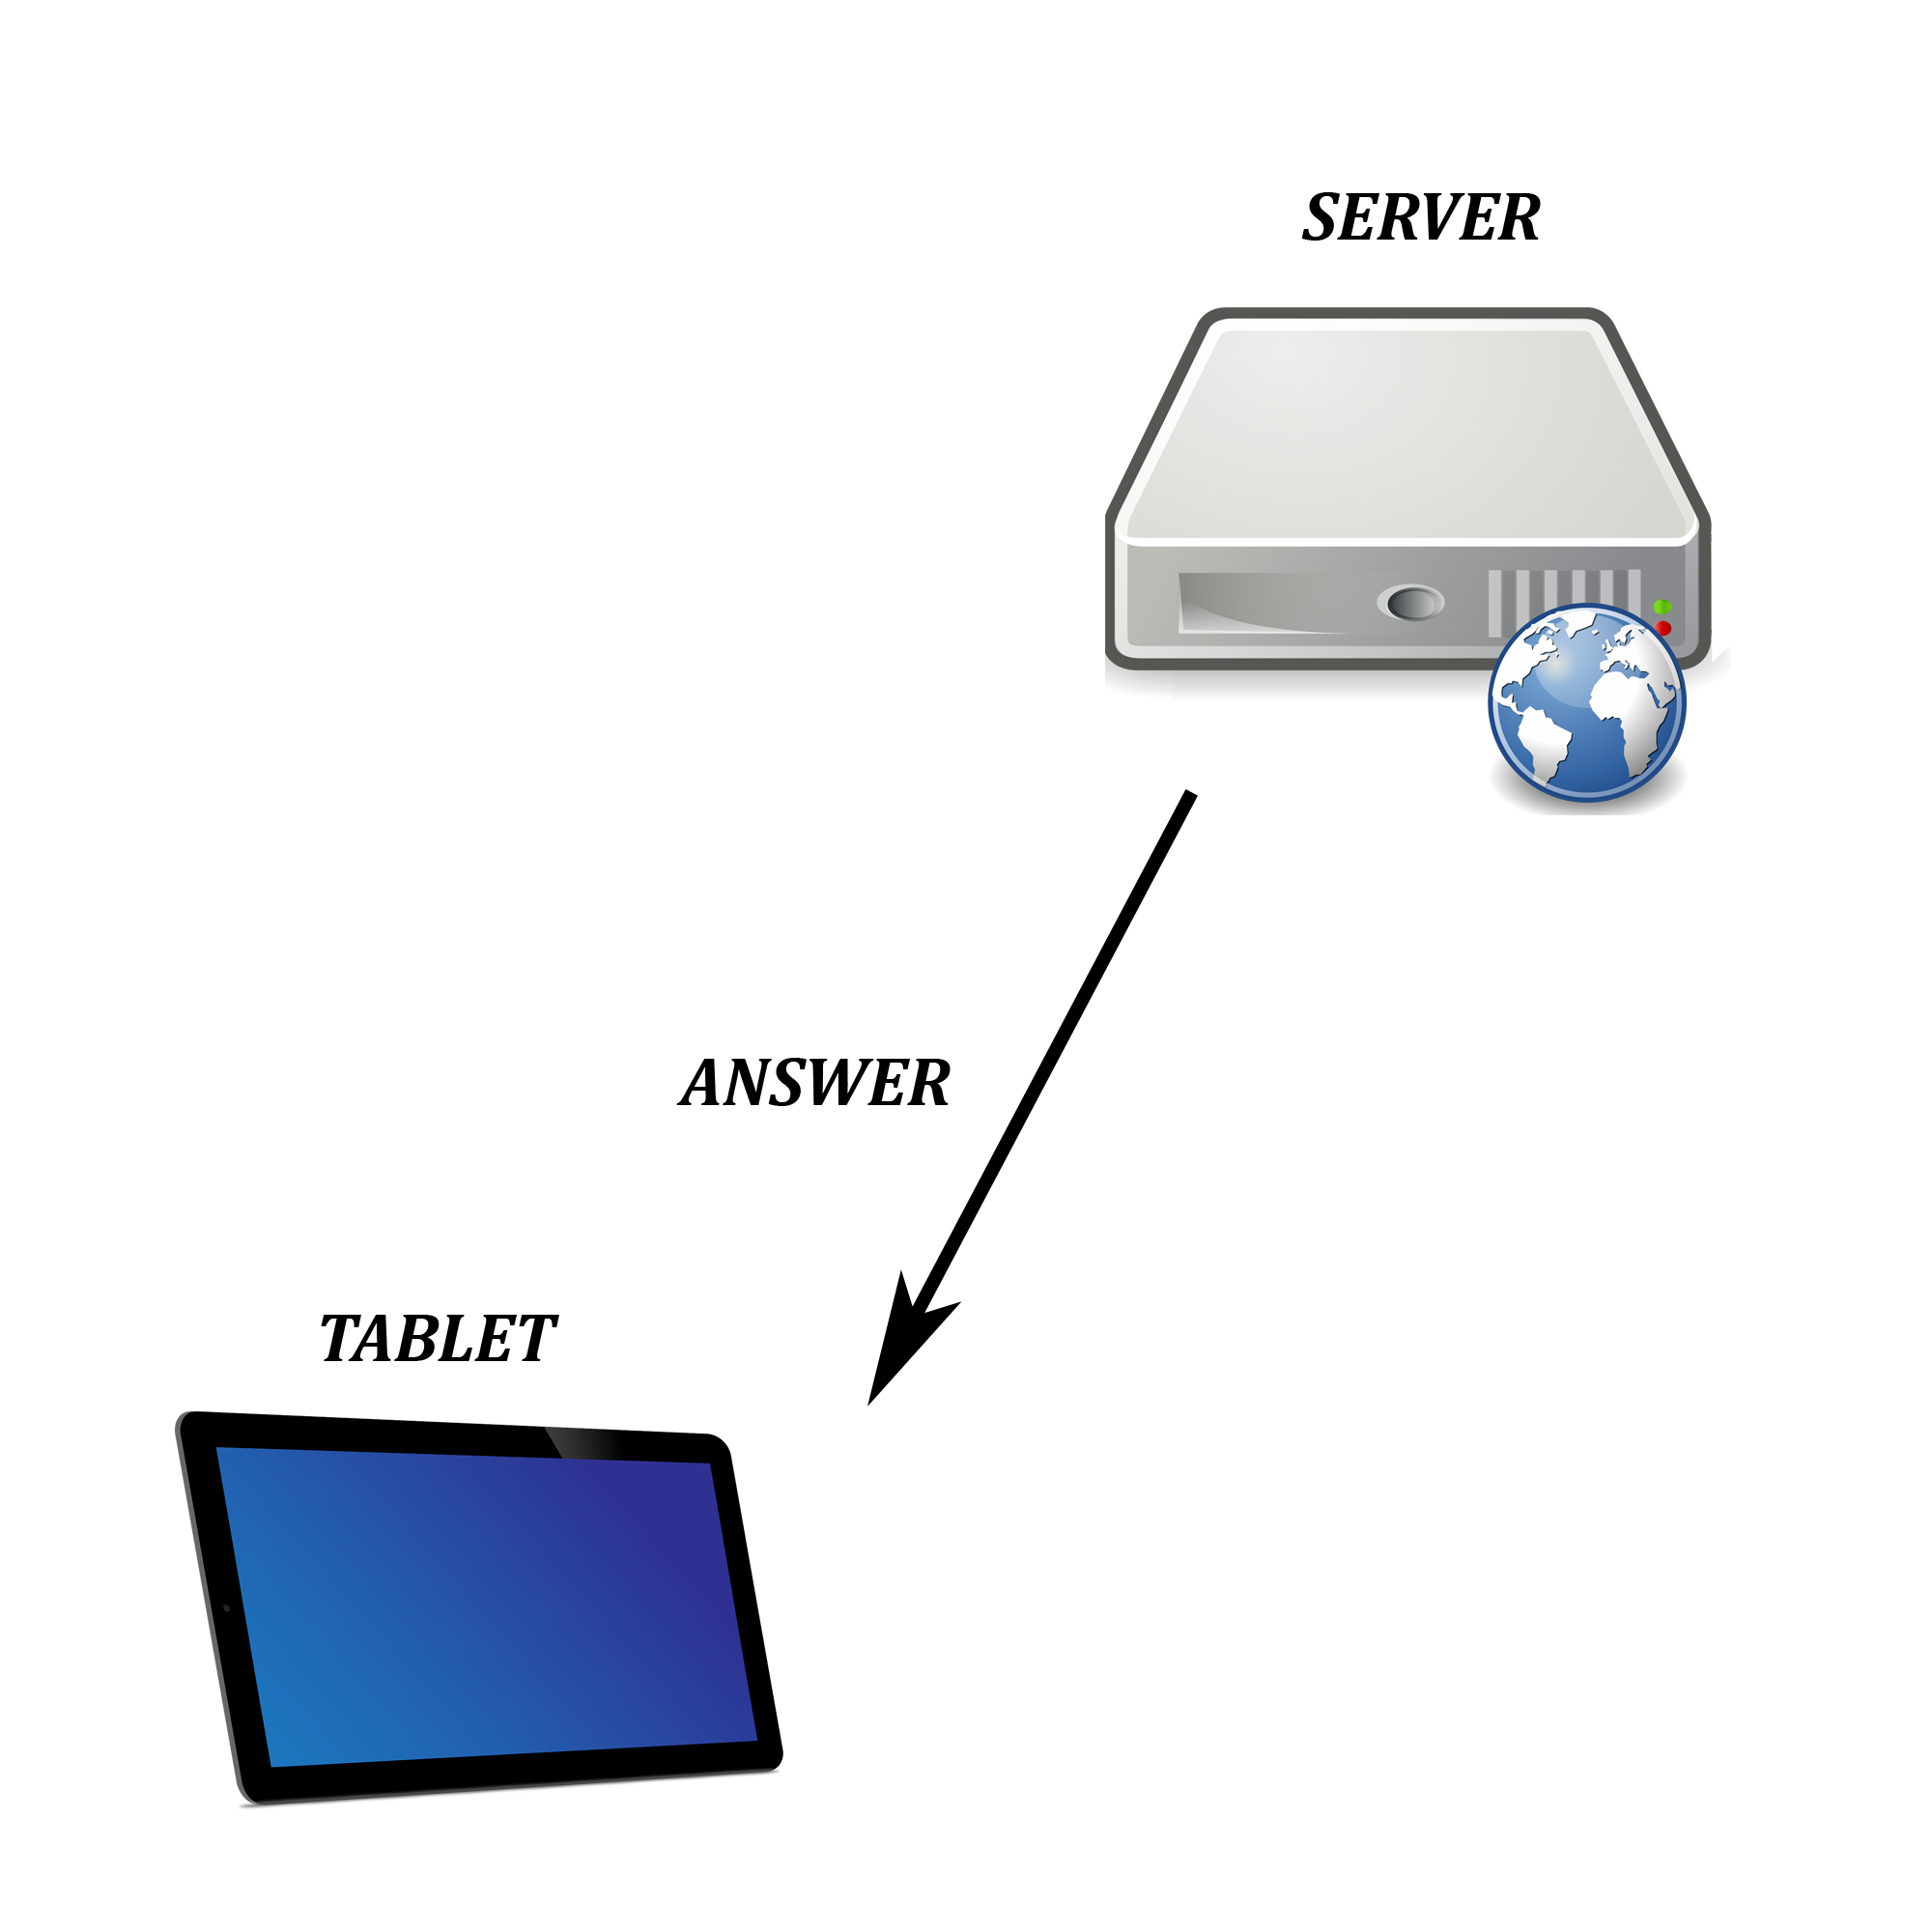
\includegraphics[height=205pt]{images/network/answer.png}}
			\end{frame}
			
			\begin{frame}{How does it work?}
				\centerline{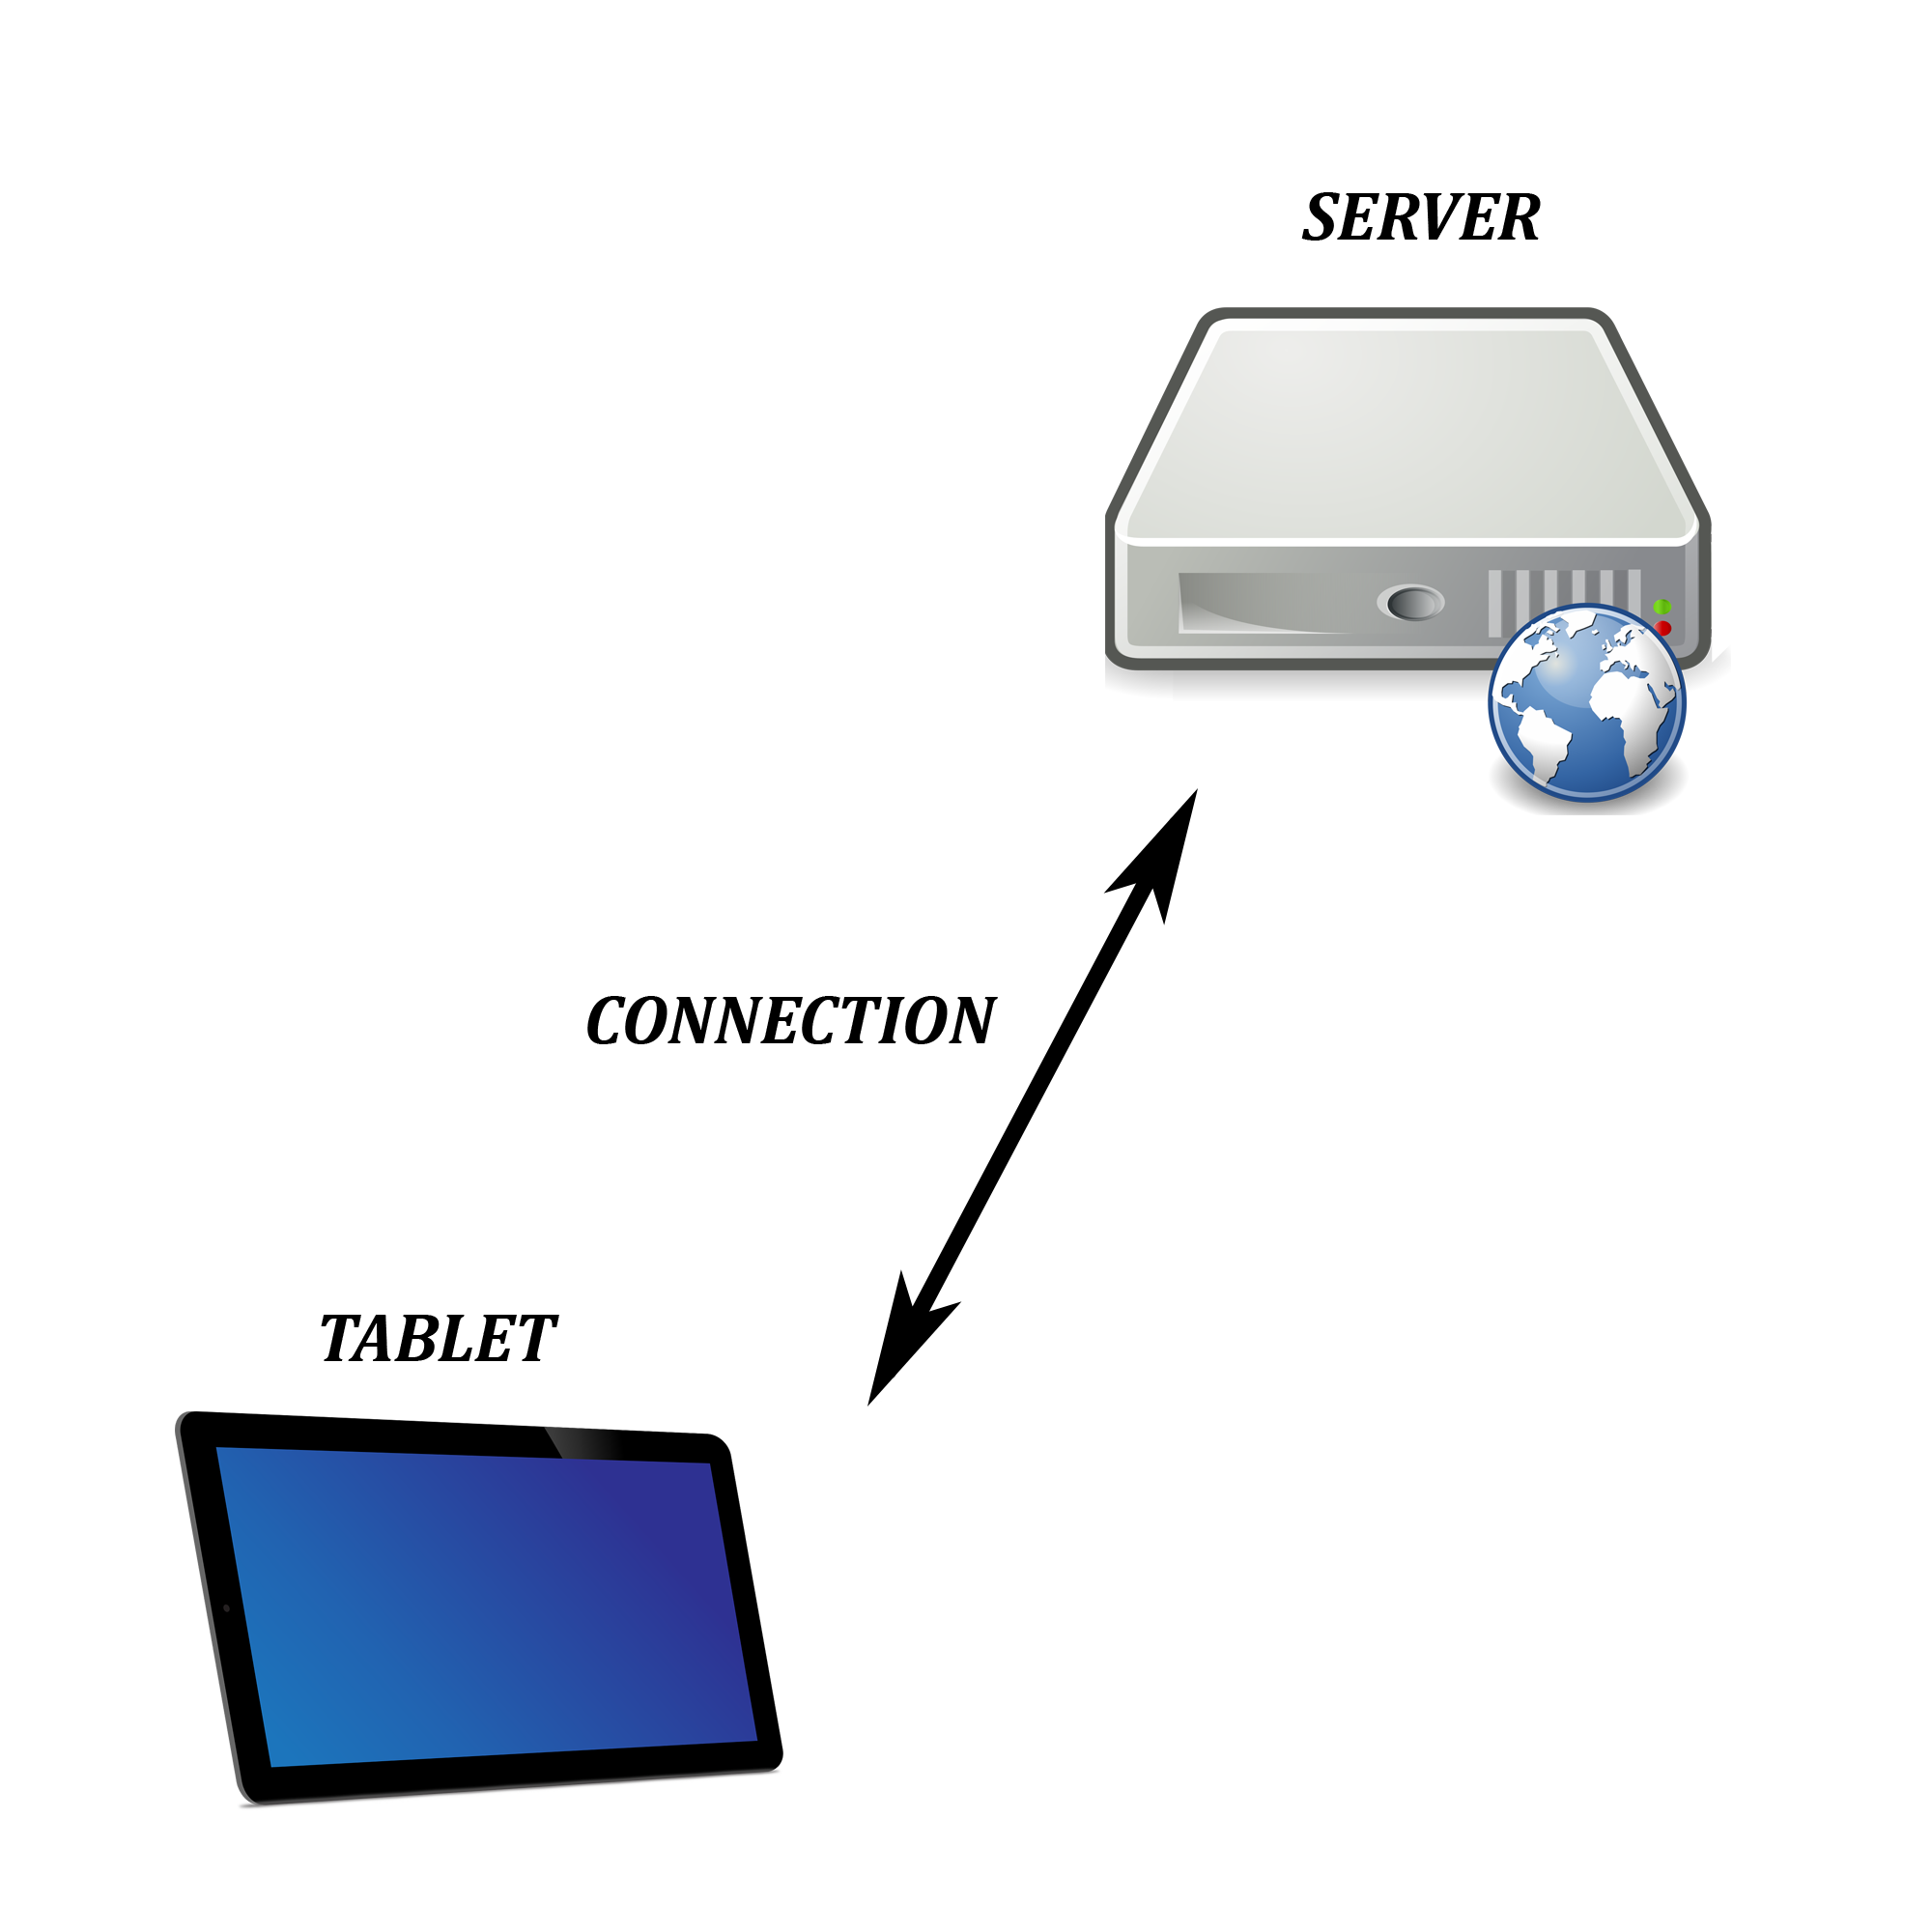
\includegraphics[height=205pt]{images/network/connection.png}}
			\end{frame}
			
			\begin{frame}{How does it work?}
				\centerline{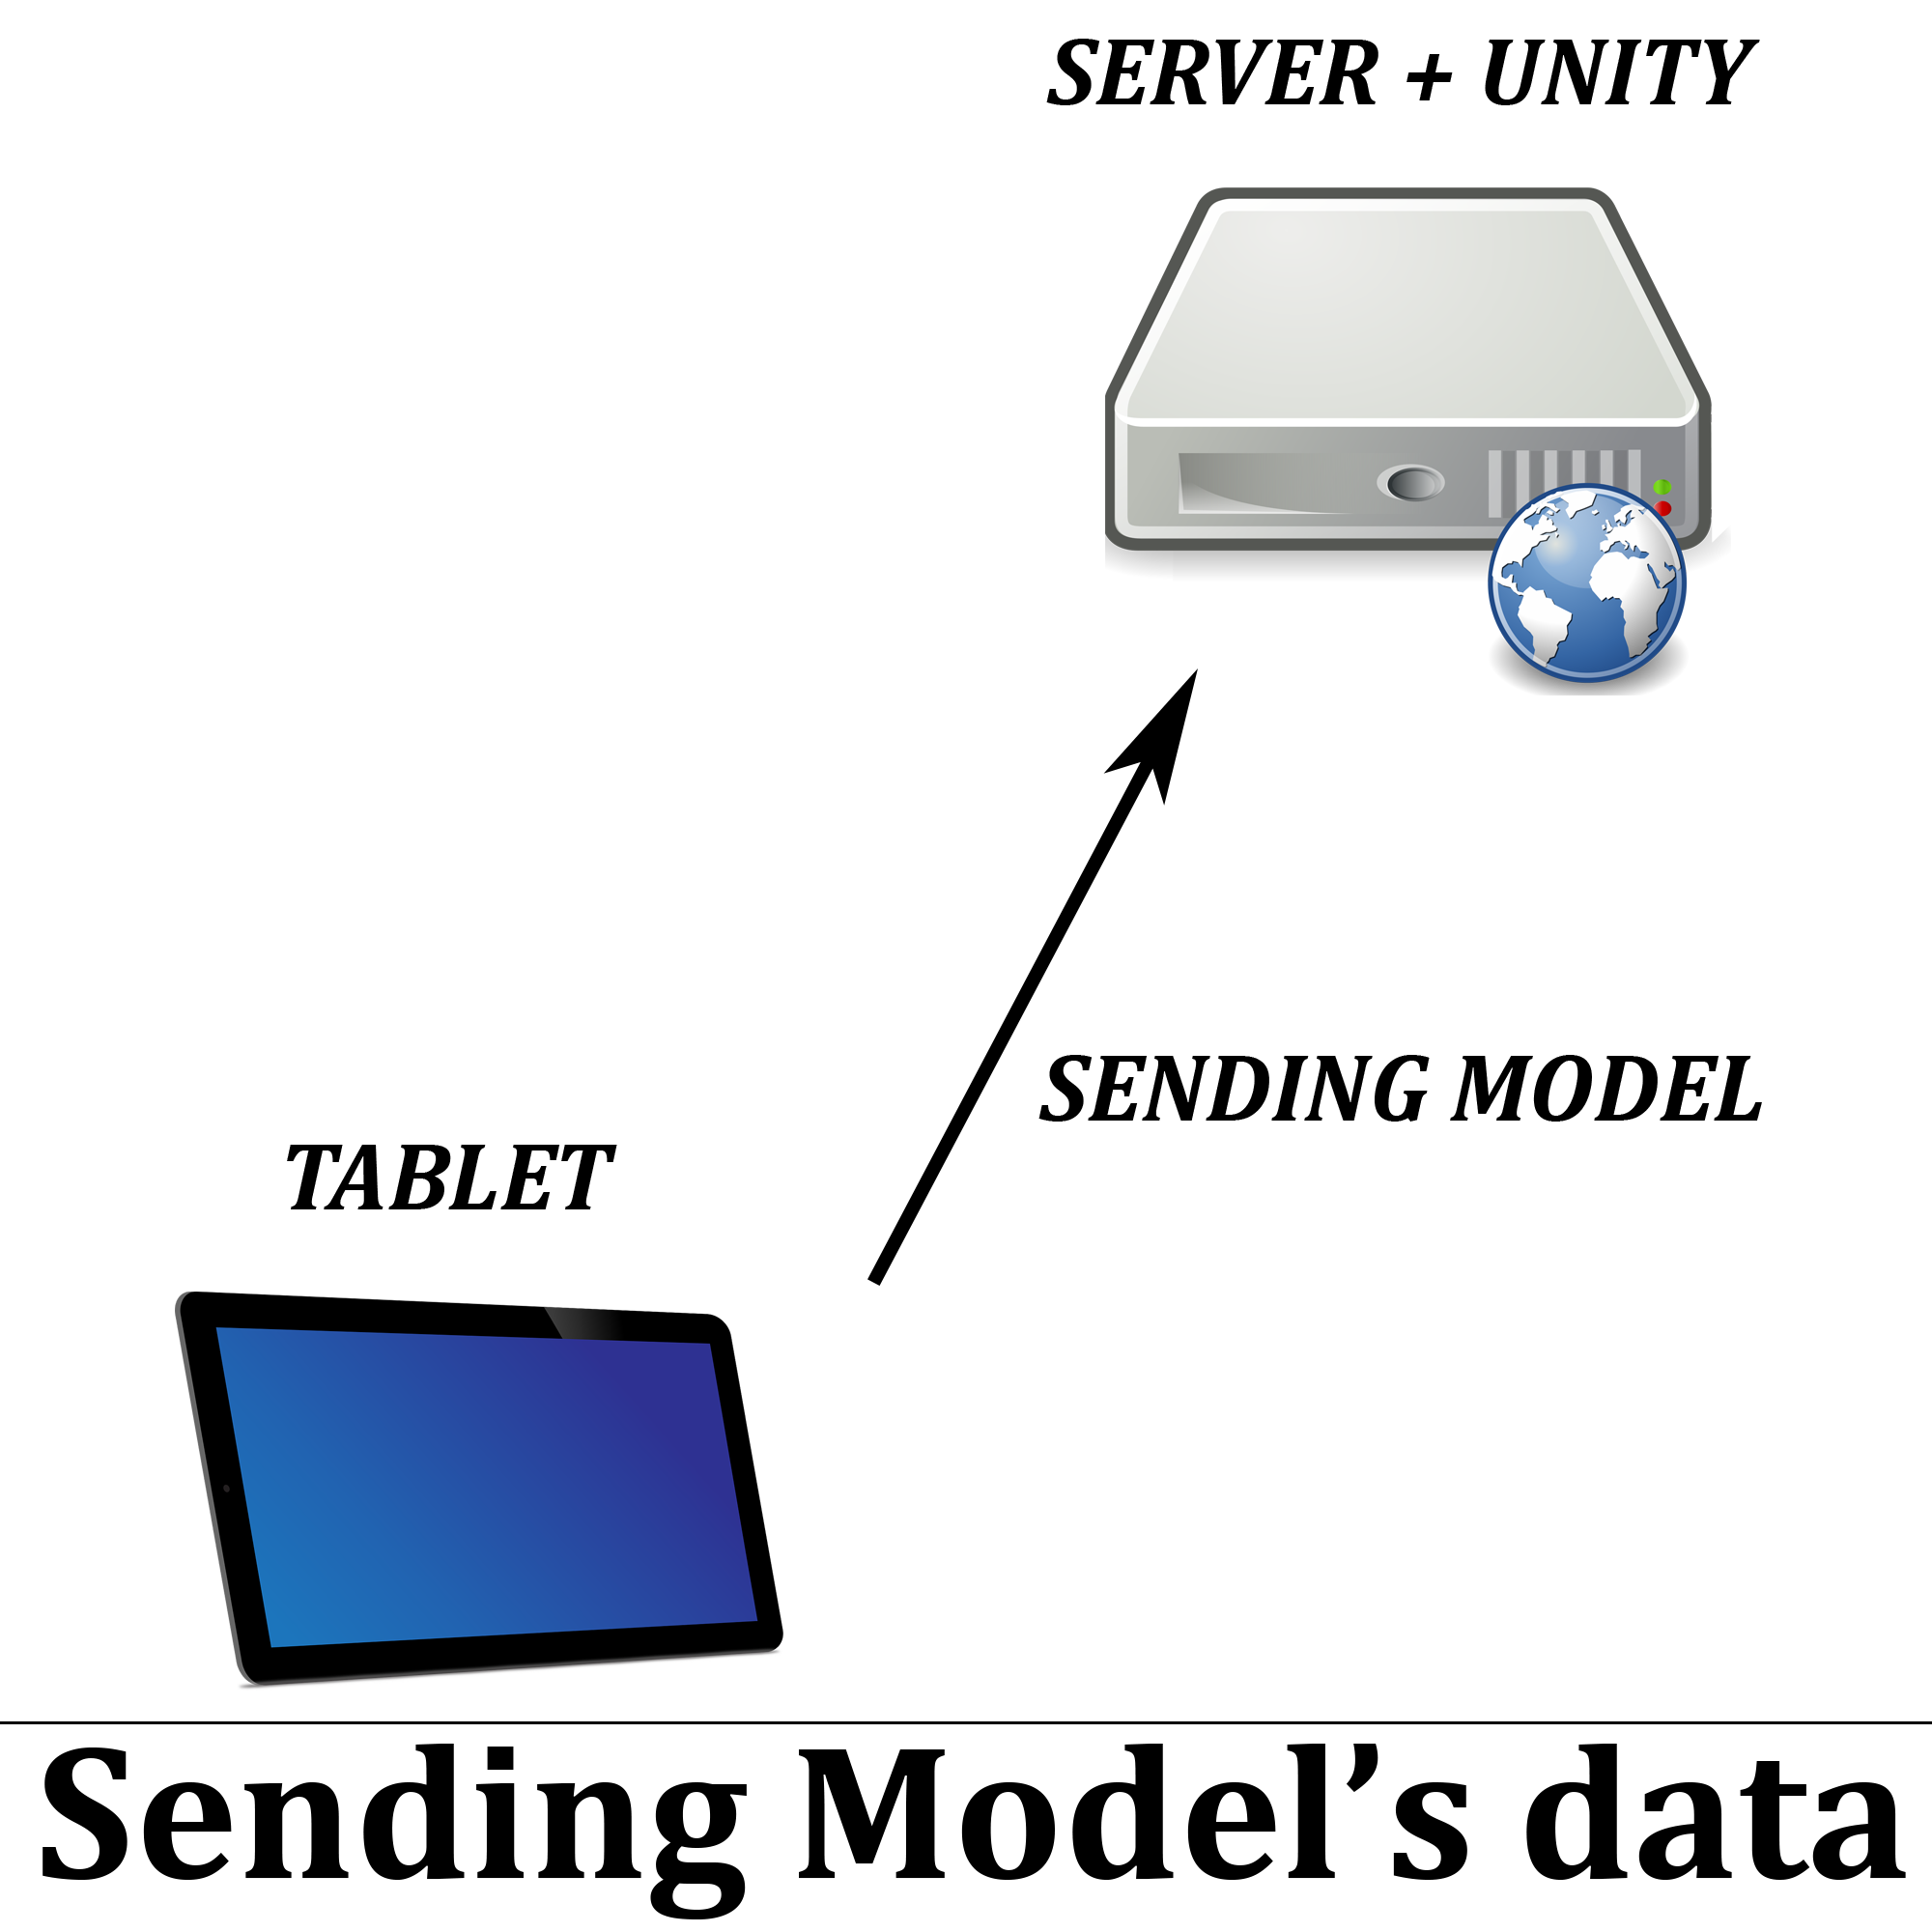
\includegraphics[height=205pt]{images/network/sending_model.png}}
			\end{frame}
		
		\subsection{External Application?}
		
			\begin{frame}{External Application?}
				\centerline{
\includegraphics[height=100pt]{images/network/no.png}}
				\begin{itemize}
					\item HTTP (HyperText Transfert Protocol)
					\item FTP (File Transfert Protocol)
				\end{itemize}
			\end{frame}
		
		\subsection{Framework}
		
			\begin{frame}{Framework}
				\centerline{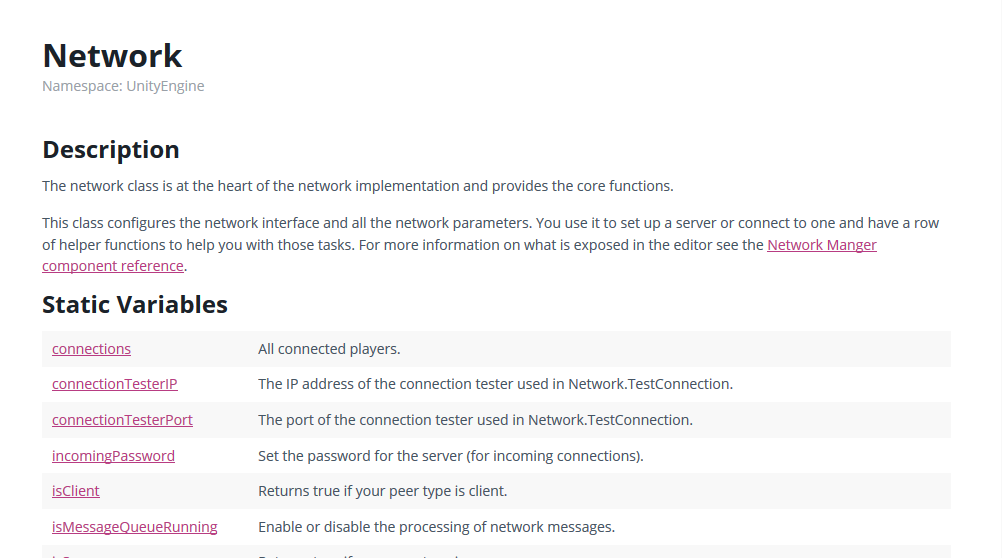
\includegraphics[height=150pt]{images/network/networkclass.png}}
			\end{frame}
	
	\section{Conclusion}
	
		\begin{frame}{Conclusion}
			\centerline{
\includegraphics[height=100pt]{images/conclusion/loupe.png}}
			\begin{itemize}
				\item Modify the interface ?
				\item improve knowledge on the Network class
			\end{itemize}
		\end{frame}
\end{document}
